\documentclass[a4paper,10pt]{article}
\usepackage{graphicx,wrapfig,hyperref}
\usepackage[hmargin=3.5cm,vmargin=3.0cm]{geometry}
\begin{document}

\title{TI2800 Contextproject - My Cultural Heritage \\ Requirements Analysis and Design}
\author{Sjoerd van Bekhoven\\ Tim Eversdijk \\ Herman Blanken \\ Rutger Plak \and 4014774 \\ 4005562 \\ 4078624 \\ 1358375}
\maketitle
\clearpage

\tableofcontents

\clearpage
\section{Introductie}
Het systeem zal onze gebruikers op een aantrekkelijke manier van zo nuttig mogelijke informatie gaan voorzien van verschillende monumenten. Deze doelen zullen op verschillende manieren worden bereikt. Deze manieren staan beschreven in hoofdstuk 2.

\clearpage
\section{Voorgesteld systeem}
	\subsection{Overzicht}
		\subsubsection{Front-end}
			Onze front-end gaat zich vooral focussen op 2 punten:
			\begin{enumerate}
				\item Het aantrekkelijk weergeven van de informatie die we vergaard hebben van de monumenten.
				\item Het systeem zo intuatief mogelijk laten werken en weergeven.
			\end{enumerate}
				
		\subsubsection{Back-end}
			Onze back-end gaat zich vooral focussen op het vergaren van nieuwe informatie voor ons systeem. Dit zal gaan gebeuren op meerdere manieren:
			\begin{itemize}
				\item Niet alle monumenten hebben standaard al een categorie aan zich gelinkt. Onze back-end zal d.m.v. beeld informatie alsnog proberen te bepalen aan wat voor categorie het monument gelinkt moet worden.
				\item Er zullen automatisch foto�s van de monumenten van de website flickr.com gehaald worden.
				\item Er zal automatisch data en foto�s van de website rijksmonumenten.nl gehaald worden.
				\item Er zullen automatisch foto�s en bijbehorende tags van de website twitter.com gehaald worden welke door user daar worden toegevoegd.
				\item Het bijhouden van user informatie.
				\item Het verwerken van user informatie tot bruikbare informatie zoals bijvoorbeeld voorkeuren van users.
				\item Het bijhouden van user interactie informatie.
			\end{itemize}
	
		\subsection{Functional requirements}	
			\subsubsection{Zoeken van relevante Flickr-foto's}
			Alle monumenten in de dataset 
			
			\subsubsection{Completeren dataset}
			Ongeveer 5000 van de ~24.500 monumenten waarover het systeem beschikt, zijn niet gecategoriseerd. Aan de hand van visuele eigenschappen van de afbeeldingen bij de monumenten en het op een nader te bepalen manier vergelijken van omschrijvingen, zal het systeem typerende criteria per categorie genereren. Aan de hand van deze criteria zullen de overige monumenten ingedeeld worden in een categorie.
				
			\subsubsection{Foursquare}
			Voor ieder van de ~24.500 monumenten zal het syteem locaties aanmaken op FourSquare. Gebruikers en overige mensen kunnen inchecken bij deze locaties. Aan de hand van de hoeveelheid check-ins bij de locaties kan het systeem een mate van populariteit calculeren. Ook mensen die het systeem niet gebruiken kunnen inchecken, waardoor de data van het syteem automatisch wordt verreikt met informatie van mensen zonder dat zij hier bewust aan meewerken.
				
			\subsubsection{Weersinformatie}
			Nog op te vullen...
				
			\subsubsection{Faciliteiten rond locatie}
			Nog op te vullen...
				
			\subsubsection{Implementeren Thesaurus}
			De nader te bepalen methode van tekstuele analyse wordt nauwkeuriger door het gebruik van een thesaurus. Tekstueel niet gelijkende woorden kunnen zeer relevant zijn. Zonder thesaurus kunnen deze links niet worden gelegd, met thesaurus kunnen hierdoor teksten op een hoger niveau worden geanalyseerd en kan er nauwkeurigere informatie worden gegeven door het systeem.
		
		\subsection{Nonfunctional requirements}
			De non-functional requirements die uitgewerkt worden zijn toegankelijkheid, onderhoudbaarheid en betrouwbaarheid.\\	\\
			\textit{Toegankelijkheid}\\
			Er is een centrale server waar alle berekeningen worden uitgevoerd met specifieke software. De client heeft slechts een internetbrowser met een v8 javascript engine. Dit betekent dat het op iedere computer / handheld met een gerenomeerde webbrowser (IE9, Google Chrome, Mozilla Firefox, Opera, Safari) werkt. Op een handheld device als een iPhone of Android toestel zal het systeem (ondanks grotere afmetingen van de website dan van het scherm) dus ook werken. Op deze manier is de applicatie voor zoveel mogelijk mensen tegelijk bruikbaar. Een gebruiker kan het systeem thuis gebruiken, maar ook op locatie (mits verbonden met internet).\\ \\
			\textit{Onderhoudbaarheid}\\
			De onderhoudbaarheid geeft aan in hoeverre het eenvoudig, moeilijk, goedkoop of duur is om het systeem in een later stadium aan te passen om aan nieuwe requirements te voldoen of fouten te herstellen. De ontwikkelomgeving die we gebruiken maakt het mogelijk op eenvoudig aanpassingen te maken aan het systeem. De onderhoudskosten zullen dan ook laag zijn.\\ \\
			\textit{Betrouwbaarheid}\\
			De data die gebruikt wordt ligt grotendeels vast in de database. De database wordt dynamisch bijgewerkt wanneer een gebruiker interfereert met het systeem. De database zal eenmaal daags gebackupped worden naar een andere server. Bij een eventuele crash van het systeem waarbij schade aan de database zou optreden zullen alleen wijzigingen van maximaal 24 uur verdwijnen. Deze wijzigingen zijn echter geen triviale informatie voor het systeem, zij zullen het systeem alleen helpen bij het accurater tonen van informatie. Wanneer een externe source crashed, zal slechts een module of feature van de website (zoals nabije hotels tonen) niet werken. Slechts wanneer Google Maps niet meer werkt, zal een grote visuele feature van de software niet beschikbaar zijn. Met een uptime van minimaal 99,99\% (bron: nodig) komt dat neer op maximaal 9 seconden per dag. Een refresh zou dit probleem al oplossen.
			
		\subsection{Constraints ("Pseudo requirements")}
			De pseudo requirements delen we onder in de serverside en de clientside:
			\begin{itemize}
				\item De serverside van de software zal draaien op een Debian Linux machine met een Apache webserver. Visuele gelijkenissen en verschillen worden onderzocht met de objectgeorienteerde programmeertaal Java. De data zal worden opgeslagen in een (My)SQL database. Voor het afhandelen van requests van de client wordt de programmeertaal PHP gebruikt.
				\item Aan de kant van de client wordt data opgehaald in HTML formaat. Hierin wordt de website opgebouwd met behulp van CSS. Om dynamisch dingen op de site te tonen of veranderen wordt javascript gebruikt.
			\end{itemize}
				
		\subsection{Analysis models}
		Nog op te vullen...	
	
	\clearpage
\section{Use case model}
		\subsection{Use case 1}
			\textit{Use case naam}\\
			Selecteren\\ \\
			\textit{Doel}\\
			Het doel is de gebruiker op een eenvoudige wijze gebruiker monumenten te laten zoeken aan de hand van verschillende criteria. De gebruiker moet aan de hand van zijn interesses de hoeveelheid monumenten verlagen zodat eenvoudig de interesses naar voren komen in de getoonde monumenten.\\ \\
			\textit{Samenvatting}\\
			Als gebruiker wil ik aan de hand van verschillende selectiecriteria de monumenten in de resultaatpagina beperken:
			\begin{itemize}
				\item Wanneer ik kaartweergave gebruik, moeten spelden verdwijnen of verschijnen afhankelijk van of de monumenten die deze spelden verantwoorden aan deze selectiecriteria voldoen.
				\item Wanneer ik overzichtsweergave gebruik, moeten rijen informatie verdwijnen of verschijnen afhankelijk vam of de monumenten die deze rijen informatie verantwoorden aan deze selectiecriteria voldoen.
			\end{itemize}
			\textit{Actoren}\\
			Gebruiker\\ \\
			\textit{Precondities}\\
			De set met getoonde monumenten is de set van alle monumenten.\\ \\
			\textit{Triggers}\\
			Deze usecase wordt getriggerd zodra de gebruiker een of meerdere selectiecriteria invult.\\ \\
			\textit{Post condities}\\
			De input van de gebruiker wordt omgezet naar een set monumenten die aan de selectie voldoen. In de kaartweergave zal dit betekenen dat de hoeveelheid spelden verminderd. In de overzichtsweergave zal dit betekenen dat de hoeveelheid informatierijen verminderd.
		
		\subsection{Use case 2}
			\textit{Use case naam}\\
			Informatie\\ \\
			\textit{Doel}\\
			Het doel is de gebruiker op een overzichtelijke en natuurlijke van informatie over het geselecteerde monument te voorzien. De gebruiker moet nuttige informatie te zien krijgen. Ook moet de gebruiker informatie te zien krijgen die de gebruiker kunnen helpen bij het bezoeken van het monument.\\ \\
			\textit{Samenvatting}\\
			Als gebruiker wil ik wanneer ik op een speld op de kaart, of informatierij in de overzichtsweergave klik, verwezen worden naar de pagina met informatie over het monument die de speld of informatierij verantwoord. Op deze pagina wil ik de informatie beschreven in 3.2.2 te zien krijgen. Ik wil een kaartje te zien krijgen waarin is ingezoomd op het monument. Op de kaart wil ik in een straal van x kilometer hotels kunnen zoeken, evenals restaurants, barretjes en andere monumenten. Ik wil dat het systeem mijn interesses bepaald en aan de hand van mijn interesses monumenten aanraadt waar ik in ge�nteresseerd ben.\\ \\
			\textit{Actoren}\\
			Gebruiker\\ \\
			\textit{Precondities}\\
			De gebruiker weet niets van het geselecteerde monument.\\ \\
			\textit{Triggers}\\
			Deze usecase wordt getriggerd wanneer de gebruiker een monument selecteerd. In de overzichtsweergave gebeurt dit wanneer een informatierij die een monument vertegenwoordigt aangeklikt wordt. In de kaartweergave gebeurt dit bij het aanklikken van een speld die een monument vertegenwoordigt.\\ \\
			\textit{Post condities}\\
			De gebruiker weet veel over het monument en heeft alle informatie die de gebruiker nodig heeft wanneer de gebruiker het monument zou willen bezoeken.
		
		\subsection{Use case 3}
			\textit{Use case naam}\\
			Mobiliteit\\ \\
			\textit{Doel}\\
			De gebruiker op locatie voorzien van informatie en het mogelijk maken foto�s toe te voegen aan het systeem.\\ \\
			\textit{Samenvatting}\\
			Als gebruiker wil ik wanneer ik op de plaats van bestemming ben aangekomen met behulp van mijn mobiele apparaat een foto kunnen uploaden / twitteren die door het systeem wordt toegevoegd aan de foto�s die bij het monument horen. Ik wil hierbij steekwoorden kunnen meegeven die door het systeem worden herkend. Wanneer ik via dit mobiele systeem een monument, hotel, bar, of ander point of interest selecteer, wil ik dat het navigatieprogramma van mijn mobiele apparaat automatisch opent, zodat ik hier eenvoudig naar toegeleid wordt.\\ \\
			\textit{Actoren}\\
			Gebruiker\\ \\
			\textit{Precondities}\\
			De gebruiker is onderweg en wil informatie opzoeken. De gebruiker heeft op zijn mobiele apparaat een internetverbinding waarmee de gebruiker het systeem kan raadplegen.\\ \\
			\textit{Triggers}\\
			De gebruiker gebruikt zijn mobiele apparaat om een monument te selecteren. Dit kan aan de hand van de selectieprocedure beschreven in usecase 1, maar ook aan de hand van een lijst favoriete monumenten die aangemaakt kan worden zoals beschreven in usecase 4.\\ \\
			\textit{Post condities}\\
			De gebruiker heeft op locatie toegang tot informatie. Het systeem heeft extra foto�s.
		
		\subsection{Use case 4}
			\textit{Use case naam}\\
			Favorieten\\ \\
			\textit{Doel}\\
			De gebruiker zijn favoriete monumenten eenvoudig terug te laten vinden.\\ \\
			\textit{Samenvatting}\\
			Als gebruiker wil ik wanneer ik een monument heb gevonden dat ik graag zou willen bezoeken of op een later tijdstip nogmaals wil bekijken, dat ik dit monument aan een lijst kan toevoegen. Deze lijst wil ik altijd kunnen raadplegen aan de hand van een gebruikersnaam en wachtwoord. Wanneer ik onderweg ben, wil ik op mijn mobiele apparaat kunnen inloggen en alle beschikbare informatie over dit monument kunnen zien. Wel wil ik zelf kunnen bepalen of andere gebruikers mijn lijst met monumenten kunnen bekijken.\\ \\
			\textit{Actoren}\\
			Gebruiker\\ \\
			\textit{Precondities}\\
			De gebruiker heeft monumenten gevonden.\\ \\
			\textit{Triggers}\\
			De gebruiker voegt een monument toe aan zijn favorieten.\\ \\
			\textit{Post condities}\\
			De gebruiker kan inloggen om zijn lijst favoriete monumenten te raadplegen.
		
		\subsection{Use case 5}
			\textit{Use case naam}\\
			Toevoegen\\ \\
			\textit{Doel}\\
			De gebruiker extra foto�s laten toevoegen aan de database.\\ \\
			\textit{Samenvatting}\\
			Als gebruiker wil ik als ik bij een monument ben een foto kunnen maken en deze op kunnen slaan in de database. Dit wil ik doen door een tweet te sturen met mijn foto erin, daarin \#cultuurapp en \#monumentid, waarbij monumentid het id is dat het systeem aangeeft dat bij het monument hoort. Ook kan een gebruiker zodra hij of zij thuis komt foto�s van een monument uploaden.\\ \\
			\textit{Actoren}\\
			Gebruiker\\ \\
			\textit{Precondities}\\
			De gebruiker is bij het monument en maakt een foto\\ \\
			\textit{Triggers}\\
			De gebruiker twittert de foto met \#cultuurapp \#monumentid.\\ \\
			\textit{Post condities}\\
			De foto is toegevoegd aan de database van foto�s die bij het monument horen.
			
	\clearpage
	\section{Use case diagram}
		\subsection{Use case descriptions plus scenarios}
		\subsection{Business object model}
		Zie figuur \ref{bom}.
		\begin{figure}[ht!]
			\centering
			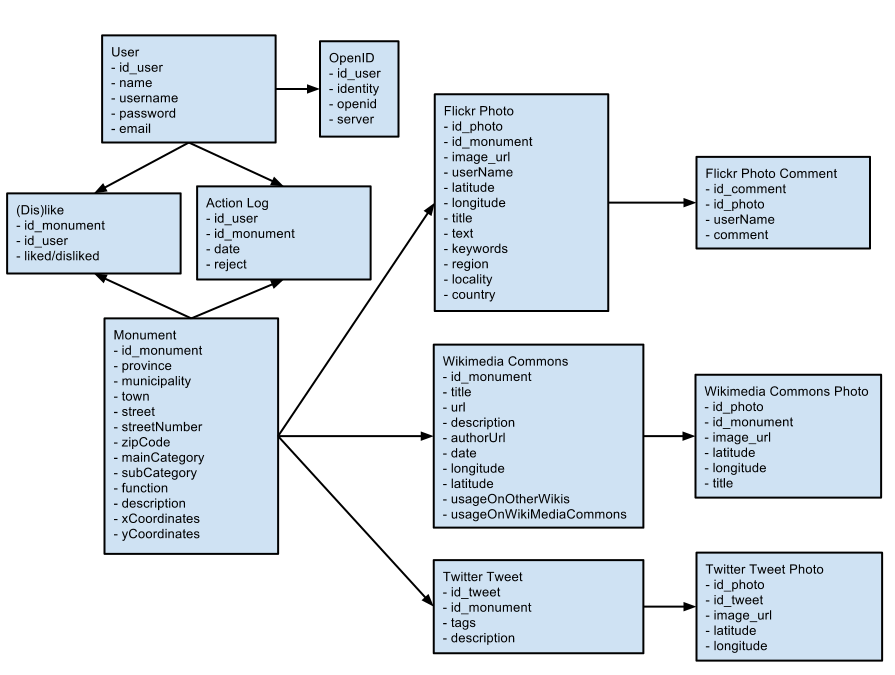
\includegraphics[width=\textwidth]{BusinessObjectModel.png}
			\caption{Business Object Model \label{bom}}
		\end{figure}
		\subsection{Dynamic models (describe the main scenarios with sequence, state, or activity diagrams)}
			\subsubsection{Sequence diagram 1}
			De gebruiker start de applicatie en komt uit op de pagina waarop de gebruiker monumenten ziet en selectiecriteria kan gebruiken, zie figuur .. %\ref{sequence1}.
			\begin{figure}[ht!]
				\centering
				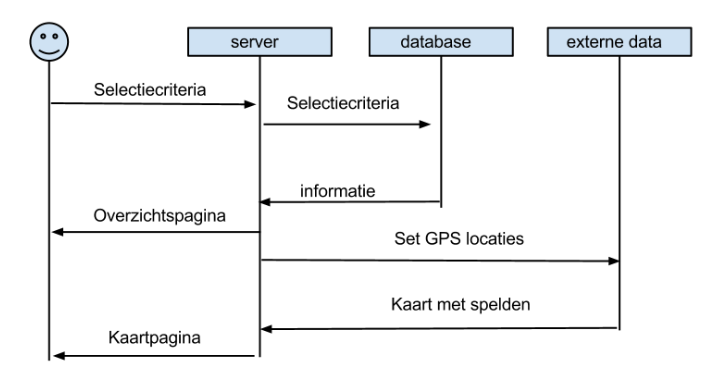
\includegraphics[width=\textwidth]{sequence1.png}
				\caption{Sequence Diagram 1 \label{sequence1}}
			\end{figure}
			\subsubsection{Sequence diagram 2}
			De gebruiker heeft een monument geselecteerd en komt uit op de detailpagina, zie figuur \ref{sequence2}.
			\begin{figure}[ht!]
				\centering
				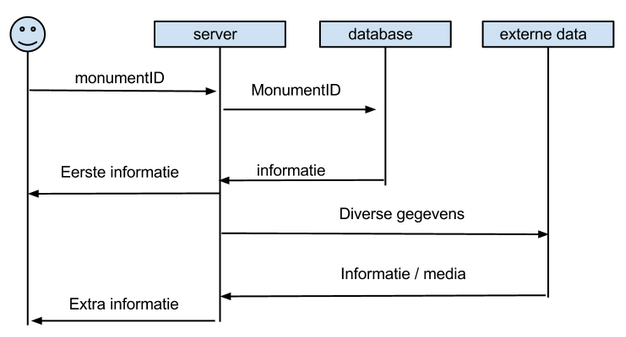
\includegraphics[width=\textwidth]{sequence2.png}
				\caption{Sequence Diagram 2 \label{sequence2}}
			\end{figure}
			\subsubsection{Sequence diagram 3}
			De gebruiker tweet een foto van een monument aan de hand van \#cultuurapp \#monumentID, zie figuur \ref{sequence3}.
			\begin{figure}[ht!]
				\centering
				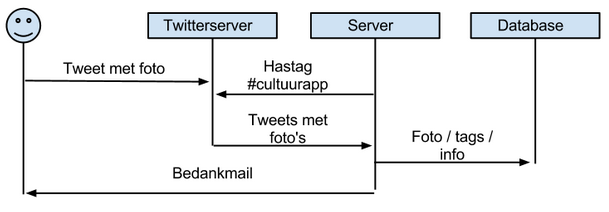
\includegraphics[width=\textwidth]{sequence3.png}
				\caption{Sequence Diagram 3 \label{sequence3}}
			\end{figure}
		
		\clearpage			
		\subsection{User interface}
			\subsubsection{Interface 1}
			De gebruiker start de applicatie en komt uit op een pagina met monumenten die de gebruiker kan filteren aan de hand van selectiecriteria. De gebruiker kan schakelen tussen twee view-mogelijkheden, namelijk de kaart met monumenten (figuur \ref{interface1}) of de overzichtspagina met monumenten (figuur \ref{interface2}). De gebruiker kan hierbij selecteren op een aantal criteria:\\
			\\
			\textit{Monmument-type}\\
			Wanneer de gebruiker het type monument wil selecteren, kan hij in een lijst van monumenttypes een of meerdere types aanvinken.\\
			\\
			\textit{Locatie}
			\begin{itemize}
				\item GPS / WIFI based huidige locatie: De huidige locatie van de gebruiker kan worden berekend door het systeem. Wanneer deze optie wordt gebruikt, wordt automatisch de �straal� ingevuld met een standaardwaarde. 
				\item Provincie / plaats / straat: De gebruiker kan in een veld een adres, straat of provincie invoeren. Wanneer deze optie wordt gebruikt, wordt automatisch de �straal� ingevuld met een standaardwaarde.
				\item Straal om de locatie: In combinatie met een gekozen locatie (ingevoerd of berekend) kan een gebied worden aangegeven waarin het systeem monumenten moet weergeven. Alleen de monumenten binnen het ingevuld aantal kilometers van de gekozen of berekende locatie worden getoond door het systeem.
				\item Te bereiken binnen x tijd met ov: Deze optie is alleen beschikbaar als er een locatie is berekend of ingevoerd. De gebruiker kan een tijdsspan invullen. Het systeem toont slechts de monumenten die binnen de ingevoerde tijdsspan met het openbaar vervoer bereikt kunnen worden.
				\item Te bereiken binnen x tijd met de auto: Deze optie is alleen beschikbaar als er een locatie is berekend of ingevoerd. De gebruiker kan een tijdsspan invullen. Het systeem toont slechts de monumenten die binnen de ingevoerde tijdsspan met de auto bereikt kunnen worden.
			\end{itemize}
			\textit{Naam}\\
			De gebruiker kan een (gedeeltelijke) naam invoeren van een monument. Alleen de monumenten met (gedeeltelijk) deze ingevoerde naam worden door het systeem getoond. Bij invoer van �abc� worden zowel monumenten �abc�, �abcdef� als �qweabc� getoond. Alle andere monumenten die de gedeeltelijke naam niet bevatten worden niet getoond.\\
			\\
			\textit{Populariteit}\\
			De populariteit van een monument wordt door het systeem berekend aan de hand van hoe vaak een monument bezocht wordt, in verhouding met hoeveel monumenten er in een straal van x kilometer ligt. Met een schuifbalk kan de gebruiker meer / minder monumenten tonen door een minimum populariteit op te geven.\\
			\\
			\textit{Trefwoorden}\\
			De gebruiker kan trefwoorden invoeren waarop de gebruiker wil zoeken. Alleen de monumenten die (in een van de bronnen) de ingevoerde woorden bevat worden getoond.\\
			\\
			\textit{Indoor/outdoor}\\
			De gebruiker kan ingeven of hij een indoor of een outdoor monument zoekt. Bij keuze van indoor worden alleen monumenten getoond die indoor zijn. Bij keuze van outdoor worden alleen monumenten getoond die outdoor zijn. Bijvoorbeeld bruggen wegen of ruines zijn leuk om te zoeken bij mooi weer. Kerken en musea zijn ook leuk om te bezoeken bij slecht weer. De categorisatie wordt gedaan aan de hand van zowel tekstuele als visuele informatie van het document.\\
			\\
			\textit{Jaartal}\\
			De gebruiker kan een range opgeven waarin het bouwjaar van een monument moet liggen. Alleen de monumenten die tussen de randwaarden zijn gebouwd worden getoond op de kaart.\\
			\\
			\textit{De input van de zoekfunctie is een set met de besproken selectiecriteria:}\\
			\{ type monument, locatie[], naam, populariteit, trefwoorden, indoor, jaartal \}\\
			\\
			\textit{De output van de zoekfunctie is een set monumenten die aan de selectiecriteria voldoen:}\\
			De gebruiker zal dit ervaren doordat slechts de set monumenten die aan de selectiecriteria voldoen op de kaart worden getoond, of in de overzichtsweergave in de lijst worden getoond.
			\subsubsection{Interface 2}
			Wanneer de gebruiker een monument heeft geselecteerd komt de gebruiker uit op een detailpagina (figuur \ref{interface3}).\\
			\\
			\textit{Details die altijd bij een monument worden weergeven:}
			\begin{enumerate}
				\item Naam, de naam van het monument.
				\item Omschrijving, een korte omschrijving van het monument.
				\item Plaatje, een plaatje van het monument uit het monumenten register.
				\item Locatie (longitude, latitude), deze zal worden weergeven d.m.v. een kaartje (google maps).
				\item Provincie, provincie waar het monument zich bevind.
				\item Gemeente, gemeente waar het monument zich bevind.
				\item Stad, stad waar het monument zich bevind.
				\item Postcode, de postcode van het gebied waar het monument zich bevind.
				\item Datum, de datum van toevoeging in het monumenten register.
				\item Categorie, de categorie van het monument.
			\end{enumerate}
			
			\begin{figure}[ht!]
				\centering
				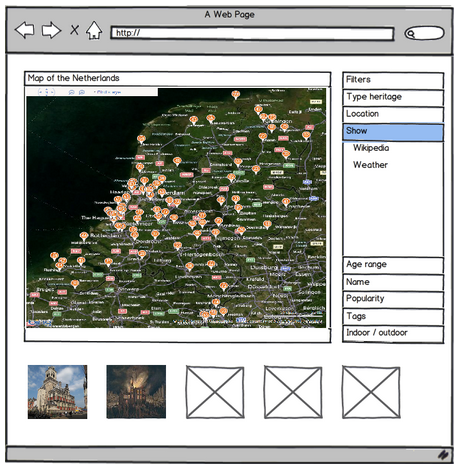
\includegraphics[height=10cm]{interface1.png}
				\caption{Kaart met monumenten \label{interface1}}
			\end{figure}
			
			\begin{figure}[ht!]
				\centering
				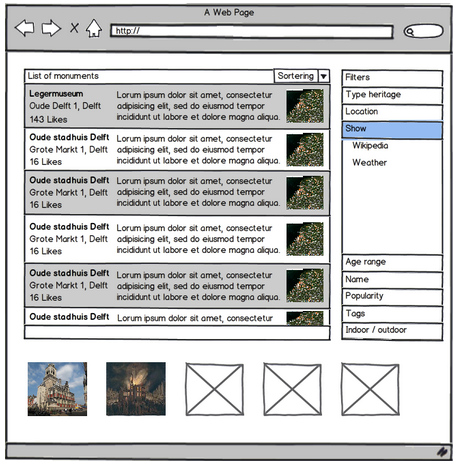
\includegraphics[height=10cm]{interface2.png}
				\caption{Overzichtspagina met monumenten \label{interface2}}
			\end{figure}
			
			\begin{figure}[ht!]
				\centering
				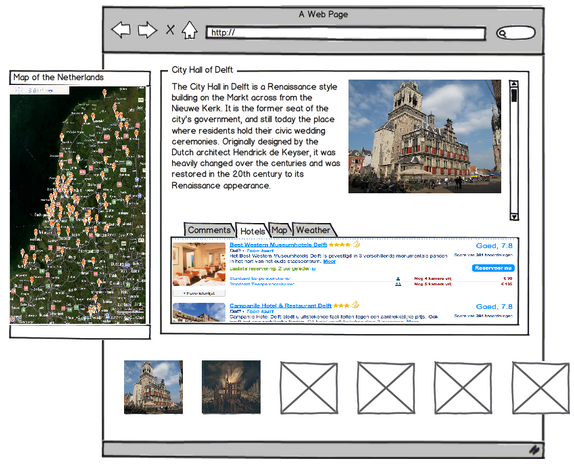
\includegraphics[height=10cm]{interface3.png}
				\caption{Detailpagina monument \label{interface3}}
			\end{figure}
			\textit{Details waarvan het systeem informatie toont wanneer deze berekend kunnen worden / beschikbaar zijn:}
			\begin{enumerate}
				\item Foto�s van het monument, op diverse manieren vergaard van diverse data-sources.
				\item Weersverwachting voor de locatie van het monument.
				\item Informatie over of het monument overdekt is, of in de open lucht.
			\end{enumerate}
	
	\clearpage
	\section{Glossary}
		\begin{itemize}
			\item towerbridge - veel besproken voorbeeld monument
			\item koffie
		\end{itemize}
\end{document}